%
% File eacl2017.tex
%
%% Based on the style files for ACL-2016
%% Based on the style files for ACL-2015, with some improvements
%%  taken from the NAACL-2016 style
%% Based on the style files for ACL-2014, which were, in turn,
%% Based on the style files for ACL-2013, which were, in turn,
%% Based on the style files for ACL-2012, which were, in turn,
%% based on the style files for ACL-2011, which were, in turn, 
%% based on the style files for ACL-2010, which were, in turn, 
%% based on the style files for ACL-IJCNLP-2009, which were, in turn,
%% based on the style files for EACL-2009 and IJCNLP-2008...

%% Based on the style files for EACL 2006 by 
%%e.agirre@ehu.es or Sergi.Balari@uab.es
%% and that of ACL 08 by Joakim Nivre and Noah Smith

\documentclass[11pt]{article}
\usepackage{eacl2017}
\usepackage{times}
\usepackage{url}
\usepackage{latexsym}
\usepackage{graphicx}

%\eaclfinalcopy % Uncomment this line for the final submission
%\def\eaclpaperid{***} %  Enter the acl Paper ID here

%\setlength\titlebox{5cm}
% You can expand the titlebox if you need extra space
% to show all the authors. Please do not make the titlebox
% smaller than 5cm (the original size); we will check this
% in the camera-ready version and ask you to change it back.

\newcommand\BibTeX{B{\sc ib}\TeX}

\title{Sanskrit Sandhi Splitting and Merging: Benchmark Datasets and Evaluation}

\author{Dr. Rahul Garg \\
 IIT Delhi \\
  New Delhi, India \\
  {\tt rahulgarg@cse.iitd.ac.in} \\\And
  Dr. Sumeet Agarwal \\
  IIT Delhi \\
 New Delhi, India \\
  {\tt sumeet@ee.iitd.ac.in} \\}

\date{}

\begin{document}
\maketitle
\begin{abstract}
	Sanskrit is one of the oldest and culturally rich languages that originated in 200 B.C. Learning the fundamentals of an old language will provide insights to the overall community of language modeling. There are two broad ways of performing language modeling: (i) Grammar model and (ii) probabilistic model. Words in Sanskrit language are formed by a process called Sandhi merging, which is a combination of two or more morphemes (component words). The reverse process of getting back the component words from the full words is known as Sandhi splitting. It is believed by many scholars that though \textit{P\={a}\d{n}ini's} has written a grammar for Sanskrit words in his monumental work called \textit{A\d{s}\d{t}\={a}dhy\={a}y\={\i}}. Analyzing and understanding word formation in Sanskrit is conceptually generic providing us with a framework to write grammars for other languages. However, the publicly available dataset such as the University of Hyderabad dataset is very erroneous making it challenging to evaluate automated algorithms. The primary contribution of this research work is to create a set of golden datasets with manually created ground truth made public for promoting open research in this fundamental problem. Further as the second contribution, we present the results of three publicly available tools for performing Sandhi splitting and Sandhi merging and benchmark their performance. We finally discuss the characteristics of each of the tool and emphasize the need for further research.
\end{abstract}

\section{Introduction}

The basic constituents of a language are its characters which are joined together to form morphemes, which is the meaning fundamental part of a language that cannot further divided. Morphemes are combined together to form words, words are combined to form sentences, and sentences are combined to form large texts. The purpose of a language model is to understand the underlying rules and structure that comprises a language. There are two broad approaches for constructing a language model as follows:
\begin{itemize}
	\item \textbf{Grammar based model:} This approach is generally used to model complex but deterministic grammar based languages. The learning models can be rule based or typically require less training data.
	\item \textbf{Probabilistic based model:} When a deterministic grammar is not available, a probabilistic language model can be learnt using a large corpus of data.
\end{itemize}

Sanskrit is one of the oldest languages designed by mankind having its origin in the Indo-Aryan civilization from 200B.C. Sanskrit has a rich tradition of poetry and literature works written, making it an important linguistic study. Being one of the oldest language, word formation in Sanskrit can be defined by set of deterministic rules and follows a defined structure. \textit{A\d{s}\d{t}\={a}dhy\={a}y\={\i}} (meaning a collection of eight books) by \textit{P\={a}\d{n}ini} is the source of Sanskrit's grammar, syntax, and semantics. The importance of \textit{a\d{s}\d{t}\={a}dhy\={a}y\={\i}} is three fold. The first one, as is well known, as an almost exhaustive grammar for any natural language with meticulous details yet small enough to memorize. Though \textit{a\d{s}\d{t}\={a}dhy\={a}y\={\i}} is written to describe the then prevalent Sanskrit language, it provides a grammatical framework which is general enough to analyse other languages as well. This makes the study of \textit{a\d{s}\d{t}\={a}dhy\={a}y\={\i}} from the point of view of concepts it uses for language analysis important. The third aspect of \textit{a\d{s}\d{t}\={a}dhy\={a}y\={\i}} is its organization. The set of less than 4000 \textit{s\={u}tra} is similar to any computer program with one major difference the program being written for a human being and not for a machine thereby allowing some non-formal or semi-formal \textit{s\={u}tra} which require a human being to interpret and implement them. Nevertheless, we believe that the study of \textit{a\d{s}\d{t}\={a}dhy\={a}y\={\i}} from programming point of view may lead to a new programming paradigm because of its rich structure. In this way, 	\textit{P\={a}\d{n}ini's} created a brief and immensely dense work. 

<<Write about Sandhi and splitting and merging>>


\subsection{Types of Sandhi} - Sandhi can take place either within a word, or between two words. Thus, it is of two types:
\begin{enumerate}
\item \textbf{Internal Sandhi:} Sanskrit grammar has three kinds of minimal meaningful units (morphemes) – prefixes, roots and suffixes and it seems that every word in Sanskrit can be derived from them. When these units combine to form a word, \textit{sa\d{m}hit\={a}} applies and certain changes take place. This is known as internal sandhi.
For example, \textit{ bho} (changed form of verb \textit{bh\={u}} bhuu (‘’to be’’)) + \textit{anam} (anam, a noun forming suffix) $\rightarrow$ \textit{bhavanam }(bhavanam, “being”) is a case of internal sandhi.

\item \textbf{External Sandhi:}
When sandhi takes place between two words, it is known as external sandhi. For example,
\textit{tau} (``both of them'') + \textit{ekad\={a}} (``once'') $\rightarrow$ \textit{t\={a}vekad\={a}} (``both of them once'') involves external sandhi.

\end{enumerate}



    
Also, depending on whether the two letters that are combining are vowels, consonants or visarga, sandhis are classified as follows:
\begin{enumerate}
\item \textbf{Vowel Sandhi:} Both letters are vowels e.g. \textit{ hima} (``snow'') + \textit{ \={a}laya\d{h}} (``house'') $\rightarrow$ \textit{him\={a}laya\d{h}} (``house of snow'')
\item \textbf{Consonant Sandhi :}  At least one of the two letters is a consonant, e.g. \textit{v\d{r}k\d{s}a} (``tree'') + \textit{ch\={a}y\={a} }(``shade'') $\rightarrow$ \textit{v\d{r}k\d{s}acch\={a}y\={a}} (``shade of tree'') 
\item \textbf{Visarga Sandhi :} A visarga combines with a vowel or a consonant, e.g.  \textit{ puna\d{h} }(``again'') + \textit{janma }(``birth'') $\rightarrow$ \textit{punarjanma} (punarjanma, “rebirth”)

\end{enumerate}


\subsection{Sandhi Splitting}
The process of breaking a sandhied word into the original units it is made of is known as sandhi splitting. A tool which can perform this task is referred to here as a sandhi splitter.
\subsection{Sandhi Merging}
On the other hand merging of two or more words into a compound word is refereed to Sandhi Merging.

\section{Exisiting Sandhi Splitting and Merging tools:}
The process of breaking a sandhied word into the original units it is made of is known as sandhi splitting. A tool which can perform this task is referred to here as a sandhi splitter.  In the same lines the tools which can merge two words to form the compound word is known as sandhi merging tool. 
There has been considerable amount of research in the field of sandhi splitting and merging. As of now, three distinct sandhi splitters and merging tools are available:



\subsection{Sanskrit Sandhi Analyzer and Splitter}\footnote{\url{http://sanskrit.jnu.ac.in/rstudents/mphil/sachin.pdf}} This is a vowel-sandhi splitter. The other two kinds of sandhis (consonant and visarga) are not split by this. This was developed at Jawaharlal Nehru University under the guidance of Prof. Girish Nath Jha (Professor, Computational Linguistics, Special Centre for Sanskrit Studies). This is available at \url{http://sanskrit.jnu.ac.in/sandhi/viccheda.jsp}.

Architecture of the system is as follows:

\subsubsection{Pre-processing}
Pre-processing includes marking the punctation marks, check the word length to determine whether we can split the words or not, and searching in the corpus if the intput word is already an instance of the examples.

\subsubsection{Subanta analysis}
This analysis includes splitting the noun phrases into its constituents base (prātipadika) and case terminations (kāraka-vacana-vibhakti).  Sandhi analyzer  will  process  the  base  words only. 

\subsubsection{Fixed List checking}
	After  subanta analysis, the input text has been segmented into base and affixes. Now only  base  words  will  be  processed  for  sandhi analysis.  But  before  that  these  words  will  be  checked  into  a Dictionary (Monier Williams Sanskrit Digital Dictionary),  place  name  list  and  noun  list.  The  words  found  in  these  resources, will  be exempted  from  sandhi processing. These different files are  merged to  one text file which is named as lexicon.
	
\subsubsection{Sandhi Analysis}
The segmenter class will check the  vowel sandhi rule - base in the database to mark the resultant  sandhi sounds  (marker)  for  potential  splitting  and  to  identify  the  sandhi patterns  for  viccheda , corresponding to the marked sound. 


\subsubsection{Result generator}
	At  each  step  of  marker  and  pattern  identification,  the  class  will  check  the  segmented  words  in  the  lexicon  to  generate  the  result.  For  this  purpose,  it  will  use  Dictionary (Monier Williams Sanskrit Digital Dictionary)  and  customized Sanskrit corpora as the ling uistic resources. To be a valid segmentation , both  the segments must be available in either of the linguistic resources. If the word has more  than one sounds marked for  sandhi , then only the first word must be present in either of  the linguistics resources . The remaining string in this case will continue with the process  of rule pattern matching, splitting and search in the linguistic resources.


\subsection{Sandhi-Splitter} This was developed at University of Hyderabad under the guidance of Ms. Amba Kulkarni (Associate Professor, Department of Sanskrit Studies). This is available at \url{http://sanskrit.uohyd.ac.in/scl/}  . 
Another Sandhi splitter is available at the TDIL website 
\url{http://tdil-dc.in/san/sandhi_splitter/index_dit.html}  but it is the same as the one mentioned above, the only difference being in version. The former is considered here because it is the latest version.

\subsubsection{Segmentation Algorithm}
The basic outline of the algorithm is\cite{Kumar2010}:
\begin{enumerate}
	\item Recursively break a word at every possible position applying a sandhi rule and generate all possible candidates for the input.
	\item Pass the constituents of all the candidates through the morphological analyser.
	\item Declare the candidate as a valid candidate, if all its constituents are recognised by the morphological analyser, and all except the last segment are compounding forms.
	\item Assign weights to the accepted candidates and sort them based on the weights as defined in the previous subsection.
	\item The optimal solution will be the one with the highest weight.
\end{enumerate}


\subsection{The Sanskrit Reader Companion } This is a Sasnkrit segmenter and parser, and therefore, also able to split sandhis. This was developed at INRIA, France under the guidance of Professor Gerard Huet, emeritus Professor. This is available at \url{http://sanskrit.inria.fr/DICO/reader.fr.html}.

 The flow of Sanskrit parser is as follows

At first the lexicon is analysed, to gather stems and their morphological parameters, such as permitted genders of nominal stems, allowed present classes (\textit{ga\d{n}a}) and attested preverbs for roots. 

In second phase, more stem generation occurs for roots, accounting  for the various tenses/moods (\textit{lak\={a}ras} ), as well as absolutives and in nitives, but also participles (adjectival \textit{k\d{r}dantas} ) in 10 varieties. 

Finally, inflexional  morphology  paradigms  derive  the  in ected  forms  according  to  the morphological parameters, some of which being read from the lexicon, some of which being de ned in speci c tables. 

It is not simple to relate our paradigmatic derivations and the operations of Paninian grammar. Some stem operations relate to morpho-phonetic operations well identified in the central rules (\textit{s\={u}tras} ), such as taking the phonetic grades of \textit{gu\d{n}a} or \textit{v\d{r}ddhi}. Some are dispersed in various parts of the grammar, such as stem substitutions. Still others, such as retroflexion, occur in the  final section (\textit{trip\={a}d\={\i}} )  of  the \textit{a\d{s}\d{t}\={a}dhy\={a}y\={\i}},  which  comprises  a  list  of  rewrite  rules  which  are applied iteratively at the end of the derivation process, in some kind of phonetic smoothing'' phase. Since the forms stored in our data banks are to be matched to the surface realization of the sentence, this phonetic smoothing must be applied at the time of generation of these forms. Some careful analysis must be done in order to understand the mutual interaction of the retroflexion rules and of the external sandhi rules (which are used in segmentation in the Heritage reader). This analysis will be given in section 4.4 below. The main discrepancy between the Paninian processes and our reader operations is in the order of rewritings. Often the stras relevant to a given operation are dispersed in different sections of the \textit{a\d{s}\d{t}\={a}dhy\={a}y\={\i}} , and thus it is hard to give the trace of the needed stras . However, in many cases, one can recognize the stra operations from the computer program. A complete analysis, in the speci c case of future passive participles .


\section{Methodology of Evaluation:}
\label{sect:methodology}

The evaluation was done in two ways: Rule-based and Literature-based. 


\subsection{Rule-based}
The three splitters are evaluated against a corpus which contains at least one example for each of the Paaninian sandhi rules. This brings out how many rules are actually implemented by the splitters. There are 282 examples against 271 rules. This evaluation was done both manually and using a tool developed for this purpose. The corpus is available at ……..

For most sandhied words, each of these splitters gives a very large number of possible splits. If any of the splits for a given word matches with the correct split, the splitter is considered to have correctly identified the splits. 

While evaluating each of the three splitters for external sandhis, even if the splits are not fully correct and there is some error in the spellings of the words far away from the location where the sandhi takes place, the slightly incorrect split is still considered as correct. An example is \textit{nayanam} (the act of directing)  whose correct split is \textit{ne} (changed form of the root nee meaning ‘direct’) + \textit{anam} (a noun forming suffix)  but \textit{ne}  + \textit{anama} is also considered to be correct, even though the last letter does not have a \textit{halanta}.  Another example is \textit{prau\d{d}ha\d{h}}(fully developed, aged, etc) where both \textit{pra} + \textit{\={u}\d{d}ha\d{h}}  and \textit{pra}+ \textit{\={u}\d{d}ha} are considered correct.  However, the automated evaluation rejects the latter result in each of these cases.


This privilege has not been given to internal sandhi cases, which if the splits are only slightly wrong, there are not considered.  This is because internal sandhi is between prefixes, roots and suffixes and small mistakes in each of these has the potential to change the meaning.
There are some rules which govern combination of letters that may themselves be the results of application of other rules. An example is \textit{v\d{r}k\d{s}as }(vrik.sas, “tree”) + \textit{\'{s}ete} ( ``sleeps'') $\rightarrow$ \textit{v\d{r}k\d{s}a\'{s}\'{s}ete} (``tree sleeps'') where the split \textit{v\d{r}k\d{s}a\d{h} } +\textit{\'{s}ete}  gives the original form. So, even though the corresponding rule has to do with change of \textit{s} to\textit{ \'{s}}, the presence of \textit{visarga} is duly considered correct.

Evaluation results are summarized in the following table

\begin{table}[h]
\begin{center}
\begin{tabular}{|l|rl|}
\hline \bf Splitting tool & \bf Manual \bf & Automated \\ \hline
JNU&12.4\%&11.4\% \\
UoH&26.6\%&18.1\% \\
INRIA&19.5\%&14.5\% \\
\hline
\end{tabular}
\end{center}
\caption{\label{font-table} Evaluation Results }
\end{table}

There is a significant difference in the results for the UoH and the INRIA splitter in the two modes of evaluation. The results of manual evaluation are detailed below as per the type of the sandhi rules :

\begin{table}[h]
\begin{center}
\begin{tabular}{|p {1.1cm}| p {1.9cm}| p {1.9cm}| p {1.2cm}| }
\hline \bf Splitter & \bf External Sandhi Cases (132) & \bf Internal Sandhi Cases (150) & \bf Overall \\
\hline
JNU &  21 (15.9 \%) & 14 (9.3 \%) & 12.4 \%  \\
 UoH & 48 (36.4 \%) & 27 (18 \%) & 26.6 \% \\
INRIA  &  49 (37.1 \%) &  6 (4 \%) & 19.5 \% \\
\hline
\end{tabular}
\end{center}
\caption{\label{font-table} Evaluation Results }
\end{table}

Cases not detected by any Splitter- 62 (46.9 %) for External Sandhi and 114 (74 %) for Internal Sandhi




\subsubsection{Analysis of Results}
\begin{itemize}
\item   A large number of rules have not been implemented, even if we leave aside those cases where the examples themselves can never be the first two words to start with, i. e. the cases that represent the second or subsequent stages of sandhi between two words, before the final word is obtained.
\item The internal sandhi phenomenon seems to have been neglected to a great extent. 
\end{itemize}



Sandhi Merging tool results:

\begin{table}[h]
\begin{center}
\begin{tabular}{|l|rl|}
\hline \bf Splitting tool & \bf Manual \bf & Automated \\ \hline
JNU&x\%&20.92\% \\
UoH&x\%&32.97\% \\
INRIA&x\%&51.77\% \\
\hline
\end{tabular}
\end{center}
\caption{\label{font-table} Evaluation Results }
\end{table}

\subsection{Literature-Based Evaluation:}
\label{ssec:litSurvey}

This takes into account the sandhied words which appear in actual literature. This evaluation is useful because the sandhi splitters are more likely to be used to split such words. If the performance of the splitters in splitting these words is satisfactory, one may consider neglecting the rules which these splitters have not been able to implement, because those rules may not be so frequent in use. However, a bad performance in this context is a cause of actual concern. 
Five different corpora were used for this purpose:
\begin{enumerate}
\item 150-word corpus
\item  Manually created Bhagvad Gita corpus containing nine chapters
\item  Dictionary-filtered UoH corpora
\item  Word-length filtered A.s.taadhyaayii corpus
\end{enumerate}

\subsubsection{150-word corpus}

This was created from 11 different texts. This has 50 examples from one text, and 10 examples each from the other ten texts. This is smaller in size compared to the other literature corpora, hence the evaluation for first was done both manually and using the automated tool. The other three were evaluated with the help of the tool only because of their much larger size.

\begin{table}[h]
\begin{center}
\begin{tabular}{p {1cm} p{2.5cm} p{2.5cm}}
\hline \bf  Splitter & \bf Manual Evaluation Results & \bf Automated Evaluation Results \\
\hline
JNU & $19 /150*100=12.66 \%$  & $15/150*100=10\%$\\
UoH & $105/150*100=70 \%$  & $98/150*100=65.33\%$\\
INRIA & $127/150*100=84.66 \%$  & $94/150*100=62.66\%$\\
\hline
\end{tabular}
\end{center}
\caption{\label{font-table} Evaluation Results }
\end{table}


\begin{table}[h]
	\begin{center}
		\begin{tabular}{p {1cm} p{2.5cm} p{2.5cm}}
			\hline \bf  Merger & \bf Manual Evaluation Results & \bf Automated Evaluation Results \\
			\hline
			JNU & $x \%$  & $75/150*100=50\%$\\
			UoH & $x \%$  & $129/150*100=86\%$\\
			INRIA & $x \%$  & $131/150*100=87.33\%$\\
			\hline
		\end{tabular}
	\end{center}
	\caption{\label{font-table} Evaluation Results }
\end{table}


The results of automated evaluation are reported below. The difference of ….. between the two sets of results is henceforth  considered as the error margin. This is expected to be the boost in performance of the three sandhi splitters if the corpora considered further were to be manually evaluated. Only automated evaluation has been done for them.

\subsubsection{Manually created Bhagvad Gita corpus containing nine chapters }

The sandhi-split Bhagvad Gita corpus at the UoH website had several limitations which made it unfit to be used for the purpose of automated evaluation. For example, within the first two chapters, out of the total of 431 sandhi cases, there were 41 typos, 92 cases of insufficient splits and 10 cases of even wrong splits.

Thus, a new corpus was manually created. This was done for half of Gita, i.e. for the 9 chapters.


Results of Automated Evaluation:

\begin{table}[h]
\begin{center}
\begin{tabular}{p{1.4cm} | p{1.6cm} | p{1.5cm} | p{1.5cm}}
\hline 
 & \bf JNU & \bf UoH & \bf INRIA \\ 
 \hline
 
\bf $A_1$ [157] &   2 (1.27 \%) &   76 (48.41 \%) &   114 (72.61 \%) \\
\bf $A_2$ [270] &   10 (3.70 \%) &   132 (48.89 \%) &   188 (69.63 \%) \\
\bf $A_3$ [169] &   11 (6.51 \%) &   83 (49.11 \%) &   110 (65.09 \%) \\
\bf $A_4$ [165] &   9 (5.45 \%) &   86 (52.12 \%) &   108 (65.45 \%) \\
\bf $A_5$ [113] &   4 (3.54 \%) &   52 (46.02 \%) &   76 (67.26 \%) \\
\bf $A_6$ [187] &   13 (6.95 \%) &   80 (42.78 \%) &   122 (65.24 \%) \\
\bf $A_7$ [120] &   6 (5.00 \%) &   43 (35.83 \%) &   84 (70.00 \%) \\
\bf $A_8$ [116] &   6 (5.17 \%) &   54 (46.55 \%) &   79 (68.10 \%) \\
\bf $A_9$ [135] &   1 (0.74 \%) &   44 (32.59 \%) &   91 (67.41 \%) \\
\bf Total [1432] &   62 (4.33 \%) &   650 (45.39 \%) &   972 (67.88 \%) \\
 
\hline
\end{tabular}
\end{center}
\caption{\label{font-table} Evaluation Results }
\end{table}


\begin{figure}[h]
	\center
	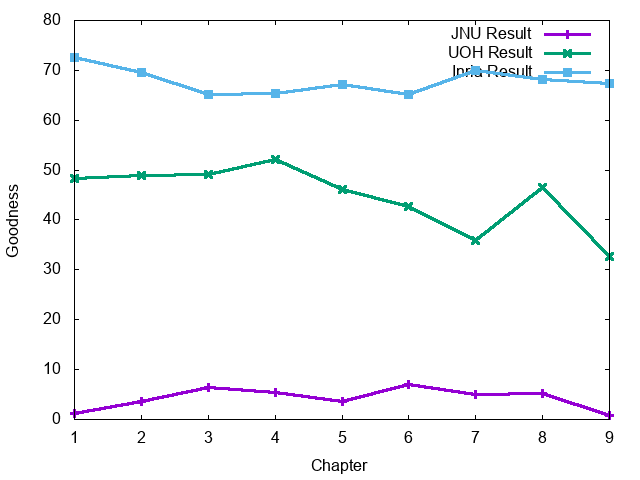
\includegraphics[scale=0.34]{images/split.png}
	\caption{\label{screen}Screenshot of the built QA system showing the orchestration flow for the question - ``problem with transfer order"}
\end{figure}

\begin{table}[h]
	\begin{center}
		\begin{tabular}{p{1.4cm} | p{1.6cm} | p{1.5cm} | p{1.5cm}}
			\hline 
			& \bf JNU & \bf UoH & \bf INRIA \\
			\hline
			
			
			\bf $A_1$ [157] &   47 (29.94 \%) &   90 (57.32 \%) &   87 (55.41 \%) \\
			\bf $A_2$ [270] &   71 (26.30 \%) &   181 (67.04 \%) &   174 (64.44 \%) \\
			\bf $A_3$ [169] &   52 (30.77 \%) &   126 (74.56 \%) &   111 (65.68 \%) \\
			\bf $A_4$ [165] &   47 (28.48 \%) &   121 (73.33 \%) &   105 (63.64 \%) \\
			\bf $A_5$ [113] &   29 (25.66 \%) &   77 (68.14 \%) &   64 (56.64 \%) \\
			\bf $A_6$ [187] &   47 (25.13 \%) &   114 (60.96 \%) &   100 (53.48 \%) \\
			\bf $A_7$ [120] &   29 (24.17 \%) &   64 (53.33 \%) &   53 (44.17 \%) \\
			\bf $A_8$ [116] &   30 (25.86 \%) &   67 (57.76 \%) &   63 (54.31 \%) \\
			\bf $A_9$ [135] &   27 (20.00 \%) &   65 (48.15 \%) &   55 (40.74 \%) \\
			\bf Total [1432] &   379 (26.47 \%) &   905 (63.20 \%) &   812 (56.70 \%) \\
			\hline
		\end{tabular}
	\end{center}
	\caption{\label{font-table} Evaluation Results }
\end{table}

\begin{figure}[h]
	\center
	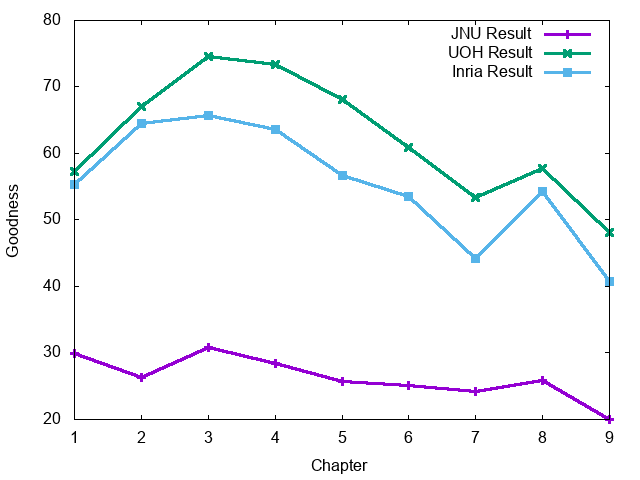
\includegraphics[scale=0.34]{images/merge.png}
	\caption{\label{screen}Screenshot of the built QA system showing the orchestration flow for the question - ``problem with transfer order"}
\end{figure}


\subsubsection{Dictionary-filtered UoH corpora}
 The UoH website has 39 sandhi-split corpora but they are not fully correct. There are cases of typos, insufficient splits and even wrong splits. Therefore, they were not directly used for the purpose of automated evaluation. The corpora contained thousands of words in total, and a strategy was worked out to create a subset of them that had no errors.
 
The strategy involved checking whether the splits could be located in some dictionary. Five dictionaries were used for this purpose. We restricted ourselves only to such cases where the splits could be located, even though they may be many cases of correct splits where the splits themselves cannot be located in the dictionary, because of various reasons (dictionaries may not contain all the declensions/ conjugations of a word, nor they are expected to). Further to check that the sandhied words in such cases did not have typos, a sandhi tool was used to do sandhi of the splits identified in the dictionary and check whether the result in each case matched with the sandhied word as given in the corpus. If the two words did not match for a particular case, it was neglected.

Just to illustrate this, we consider the five cases listed below.\\
\textit{ tumulo vyanun\={a}dayan $\rightarrow$ tumula\d{h}+vi+anun\={a}dayan\\
sarv\={a}nbandh\={u}navasthit\={a}n $\rightarrow$ sarv\={a}n + bandh\={u}n + avasthit\={a}n\\
\'{s}abda iva $\rightarrow$ \'{s}abda\d{h}+  iva\\                                              
n\={a}rhati $\rightarrow$ na + arhati\\
astamito bhagav\={a}n $\rightarrow$ astam + ita\d{h} + bhagav\={a}n
}

The first two cases were not included because at least one word in each of the splits could not be located in any of the dictionaries used for this purpose. The last three cases were considered for the purpose of evaluation. 


Results:
Total Number of Cases: 18,326


\begin{table}[h]
\begin{center}
\begin{tabular}{| r | r | }
\hline  \bf Splitter & \bf No. of Cases Correctly Identified \\
\hline
JNU & 3214 (17.53 \%) \\
UoH & 11405 (62.23 \%) \\
INRIA & 13416 (73.20 \%)\\
\hline
\end{tabular}
\end{center}
\caption{\label{font-table} Evaluation Results }
\end{table}


\begin{table}[h]
	\begin{center}
		\begin{tabular}{| r | r | }
			\hline  \bf Merger & \bf No. of Cases Correctly Identified \\
			\hline
			JNU & 6517 (35.56 \%) \\
			UoH & 12895 (70.36.2 \%) \\
			INRIA & 12611 (68.81 \%)\\
			\hline
		\end{tabular}
	\end{center}
	\caption{\label{font-table} Evaluation Results }
\end{table}


\subsubsection{Word-length filtered \textit{\={a}staadhyaayi} corpus}
    Many \textit{sutr\={a}} (rules) of \textit{p\={a}\d{n}ini} themselves contain many sandhied words. All the sutras with their splits are available at …. This was found to be another good source which could be used for the evaluation of the three splitting tools.  However, even this source suffered with the limitation of insufficient splits.  Moreover, a very significant number of splits could not be expected to be located in any dictionary, because these were the forms of the different sets/ \textit{mahesvara sutr\={a}} that \textit{p\={a}\d{n}ini} uses to codify Sanskrit grammar, syntax and semantics. Hence, the strategy used in the previous case to limit to cases of correct splits could not be applied in this case.
    
Since the problem initially arose because of cases of insufficient splits, another strategy was worked out.  The splits which can undergo further splitting themselves are likely to be of greater length than those cases in which further splitting is not possible. The larger the length of the splits, the more likely they are to undergo further splitting. All those cases where the length of the splits was less than a specified word length were analysed together and the results were noted for different values of the word lengths-10,20,30, 40 and 50.

The following five examples are used here for the purpose of illustration. At least one of the splits in each of the first two cases is considerably long, and further splitting is evident.  When the word length is reduced, the possibility of further splits is also reduced, though not eliminated. So, in the next two cases, though the word length is reduced, the first split of the third case and the second split of the fourth case can themselves be further split. It is only for the last case that further splitting is not possible.

\textit{prathamacaramatay\={a}lp\={a}rdhakatipayanem\={a}\'{s}ca $\rightarrow$ prathamacaramatay\={a}lp\={a}rdhakatipayanem\={a}\d{h}+ca \\
udupadh\={a}dbh\={a}v\={a}dikarma\d{n}oranyatarasy\={a}m $\rightarrow$ udupadh\={a}t+bh\={a}v\={a}dikarma\d{n}o\d{h}+anyatarasy\={a}m \\
taddhita\'{s}c\={a}sarvavibhakti\d{h} $\rightarrow$ taddhita\d{h}+ca+ca+asarvavibhakti\d{h} \\
v\d{r}ddhir\={a}daic $\rightarrow$ v\d{r}ddhi\d{h}+\={a}daic \\
vija i\d{t} $\rightarrow$ vija\d{h}+i\d{t} \\                                                 
}

Results on \textit{\={a}staadhyaayi}
Total Number of Sutras –3,959
Sutras where Sandhi Split Applicable –2,700
    


\begin{table}[h]
\begin{center}
\begin{tabular}{ p{2cm}  r r r }
\hline  
\bf No. of letters ($\le$) & Samples & JNU & UoH \\
\hline
\bf 10 & 93 & 4(4.3) & 21(22.6) \\
\bf 20 & 571 & 10(1.75) & 100 (17.5) \\
\bf 30 & 1512 & 17(1.12) & 226(14.9) \\
\bf 40 & 2045 & 18 (0.88) & 263(12.86) \\
\bf 50 & 2302 & 18(0.78) & 263(11.42) \\
\bf All  & 2700 & 18 (0.66) & 263 (9.74) \\
\hline
\end{tabular}
\end{center}
\caption{\label{font-table} Evaluation Results }
\end{table}


\section{Sandhitype based analysis}

\begin{figure}[h]
	\center
	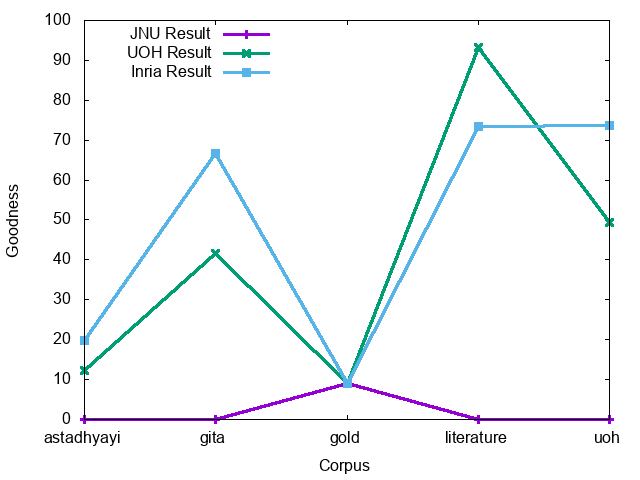
\includegraphics[scale=0.34]{images/visarga.png}
	\caption{\label{screen}Visarga}
\end{figure}

\begin{figure}[h]
	\center
	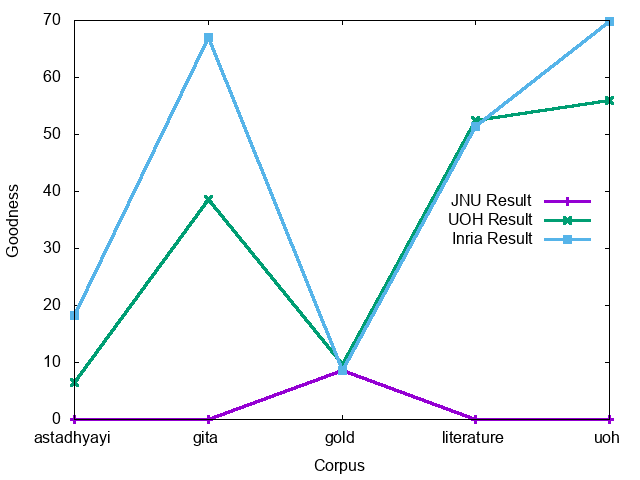
\includegraphics[scale=0.34]{images/consonant.png}
	\caption{\label{screen}Consonant}
\end{figure}

\begin{figure}[h]
	\center
	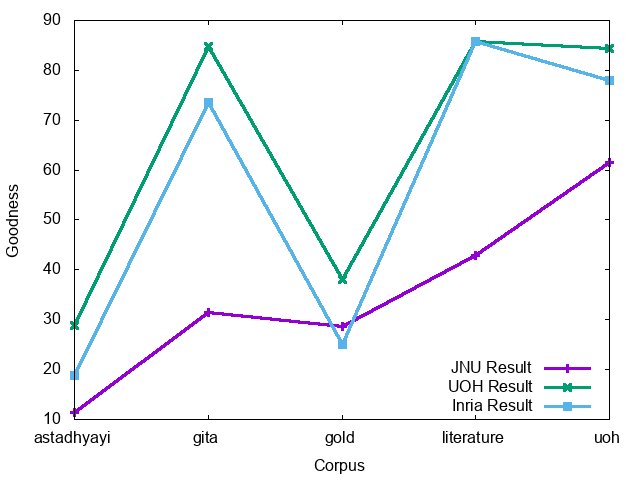
\includegraphics[scale=0.34]{images/vowel.png}
	\caption{\label{screen}vowel}
\end{figure}

\begin{figure}[h]
	\center
	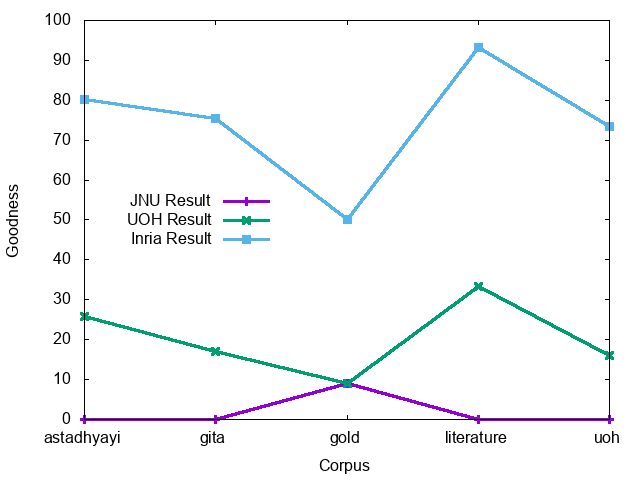
\includegraphics[scale=0.34]{images/visargamerge.png}
	\caption{\label{screen}Visarga Merge results}
\end{figure}

\begin{figure}[h]
	\center
	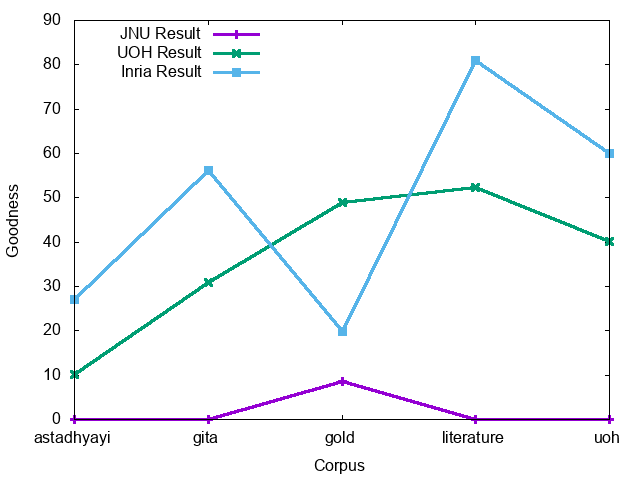
\includegraphics[scale=0.34]{images/consonantmerge.png}
	\caption{\label{screen}Consonant Merge results}
\end{figure}

\begin{figure}[h]
	\center
	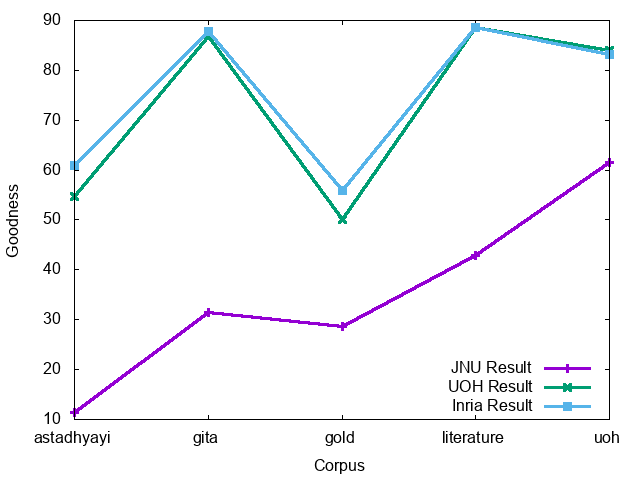
\includegraphics[scale=0.34]{images/vowelmerge.png}
	\caption{\label{screen}vowel merge}
\end{figure}




\section{Analysis of Errors}
 Literature-Based Evaluation
The literature based evaluation results are also not very impressive. The cases were looked into and the reasons behind the poor performance can be categorised as follows:


\subsection{Rules not Implemented}
      It seems that some of the rules which are even frequent used have not been implemented by one or more of the three splitters. For example, the visarga of \textit{sa\d{h}} and \textit{e\d{s}a\d{h}} is elided optionally when any letter other than \textit{a} follows it, and there are many such cases of this elision, for example, in Srimad Bhagvad Gita. But none of the three splitters is able to undo this elision to get back the visarga. For example, none of the three splitters is able to do the following split
      
                        \textit{sa yog\={\i}} $\rightarrow$ \textit{sa\d{h}} (that) + \textit{yog\={\i}} (who practises yoga)
                        
It will be incorrect to say that rules of elision, in general, are not implemented by any of the three splitters. For example, the split of
 
            \textit{b\={a}lak\={a} hasanti} $\rightarrow$ \textit{b\={a}lak\={a}\d{h}} (boys) + \textit{hasanti} (laugh) is detected correctly by INRIA.                      

    
\subsection{Optional Rules}    
There are some rules which are optional in nature, and less frequently used. For example, when \textit{e} at the end of a pada is followed by a vowel, the \textit{y} of \textit{ay} into which it changes can be optionally elided. The resultant form after elision is less common, but we do have cases in Srimad Bhagvad Gita, for example, of this kind. The following case is an example where none of the three splitters is able to detect the correct split.
    
   \textit{ vartanta iti} $\rightarrow$ \textit{vartante} (exist) + \textit{iti} (this)
   
[Had the optional rule not been applied,\textit{vartante} +\textit{iti} would have led to \textit{vartantayiti}]. 

\subsection{Cascading split effect}
There are some rules in which the effect of combination of two words is not restricted to the change in sound at the extreme boundaries of the two words (last sound of first word + first sound of second word). Other letters can also get affected. For example, in 

       \textit{uttara} (north) + \textit{ayana} (movement) $\rightarrow$ \textit{uttar\={a}ya\d{n}a} (``northward movement'', refers to movement of Sun towards Tropic of Cancer), the \textit{r} of \textit{uttara} causes the change of \textit{n} of \textit{ayana} into \textit{ \d{n}}. In absence of \textit{r}, no such change takes place in the case of 


\textit{dak\d{s}i\d{n}a} (south) + \textit{ayana} (movement) $\rightarrow$ \textit{dak\d{s}i\d{n}\={a}yana} (southward movement, refers to movement of Sun towards Tropic of Capricorn) 
The three sandhi splitters do not seem to have taken care of such changes. So, while they are able to split \textit{dak\d{s}i\d{n}\={a}yana} correctly, the same is not true for \textit{uttar\={a}ya\d{n}a}.

 Another example is the case of change of \textit{s} into \textit{\d{s}} when it is immediately preceded by some vowels (for example, \textit{i}, and this \textit{\d{s}} changing its subsequent letter because of another sandhi rule, for example  \textit{th} into \textit{\d{t}h}. Thus, we have the examples of:
 
                    \textit{prati} + \textit{sthita} $\rightarrow$ \textit{prati\d{s}\d{t}hita} (``well-established'')
                     
                     
and   \textit{yudhi} + \textit{sthira\d{h}} $\rightarrow$ \textit{yudhi\d{s}\d{t}hira\d{h}}  (one who is stable in war)
where the sandhied forms are \textbf{not split by any of the three splitters}.


\subsection{Multiple splits} 
The process of sandhi splitting involves splitting the sandhied word at different potential locations, and validating the splits to check which one of them is correct. If the set used for validation is not complete, even correct splits may sometimes not be validated. For example, in 

   \textit{a} (not) + \textit{chedya\d{h}} (``solvable'', ``penetrable'') $\rightarrow$ \textit{acchedya\d{h}} (``not solvable/penetrable'')
   
the fact that none of the three splitters has been able to split the sandhied word may have to do with the possiblity that may \textit{a} not have been validated as a proper split.


\subsection{Compounding effect}
The process of compounding, due to which words come together without necessarily their being a change when they merge, also creates problems. While the UoH and the INRIA tools do have the provision of decompounding along with sandhi splitting, the JNU splitter does not have a way to do both together.
For example,

\textit{lak\d{s}yasy\={a}rthatvavyavah\={a}r\={a}nurodhena} $\rightarrow$  \textit{lak\d{s}yasya} + \textit{arthatvavyavah\={a}ra} + \textit{anurodhena} 

The second split is not validated without decompounding, and thus even though, only vowel sandhis are involved, the JNU splitter is not able to correctly split the word.  
Even the INRIA and UoH splitters are not always able to get around this problem.
For example, none of the three splitters is able to detect this:

\textit{prapa\~{n}ce'v\={a}ntaravibh\={a}gapravibh\={a}gabhinn\={a}nantapad\={a}rthasa\.{n}kule'pi} $\rightarrow$ \textit{prapa\~{n}ce} + \textit{ava} + \textit{antara-vibh\={a}ga-pravibh\={a}ga-bhinna} + \textit{ananta-pada} + \textit{artha-sa\.{n}kule} + \textit{api}


\end{document}
